% % % % % % % % % % % % % % % % % % % % % % % % % % %
% IS&T Template 
% Patrick Vandewalle
% January 2006
% % % % % % % % % % % % % % % % % % % % % % % % % % %

%%%%%%%%%%%%%%%%%%%%%%%%%%%%%%%%%%
% Document class
%%%%%%%%%%%%%%%%%%%%%%%%%%%%%%%%%%
\documentclass[letterpaper,twocolumn,fleqn]{article} 

%%%%%%%%%%%%%%%%%%%%%%%%%%%%%%%%%%
% Packages
%%%%%%%%%%%%%%%%%%%%%%%%%%%%%%%%%%
\usepackage{ist}
\usepackage[margin=1in]{geometry}
% add other packages here
\usepackage{float} %forza
\usepackage{wrapfig} %forza
\usepackage{amsmath}
\usepackage{amssymb}
\usepackage{graphicx}
\usepackage{listings}
\usepackage{xcolor}
\usepackage{float}
\usepackage{hyperref}
\usepackage{booktabs}
\usepackage[american]{circuitikz}
\pagestyle{empty}                % no page numbers is default
\lstset{
  basicstyle=\ttfamily\footnotesize,
  breaklines=true,
  breakatwhitespace=true,
  columns=fullflexible,
  keepspaces=true,
  frame=single,
  showstringspaces=false,
  xleftmargin=0.02\columnwidth,
  xrightmargin=0.02\columnwidth
}

%%%%%%%%%%%%%%%%%%%%%%%%%%%%%%%%%%
% Title and Authors
%%%%%%%%%%%%%%%%%%%%%%%%%%%%%%%%%%

\title{Unit 1: Solution of Equations in
One Variable \\ Diode Circuit Operating Point Analysis }
\author{ Jacky Li; Cal Poly Pomona; Pomona, California \\ February 09, 2025}
 % date has an empty field.
% correct for bad hyphenation here
% \hyphenation{}

%%%%%%%%%%%%%%%%%%%%%%%%%%%%%%%%%%
% Begin document
%%%%%%%%%%%%%%%%%%%%%%%%%%%%%%%%%%
\begin{document} 
\maketitle 
\thispagestyle{empty} % prevents the first page to be numbered

%%%%%%%%%%%%%%%%%%%%%%%%%%%%%%%%%%
% Abstract
%%%%%%%%%%%%%%%%%%%%%%%%%%%%%%%%%%

\begin{abstract}
How do we find the operating point of a nonlinear circuit when no closed-form
solution exists?  
In this report we apply \textbf{Newton's method} to determine the DC operating
point of a series resistor–diode circuit governed by the Shockley diode
equation.  The resulting transcendental equation in one variable is solved
iteratively, and the convergence behaviour is compared with that of the
bisection method.  Newton's method converges quadratically---reaching
machine-level precision in fewer than 10~iterations---while bisection
requires roughly 50~iterations for the same accuracy, confirming the
well-known theoretical advantage of Newton's method for smooth, well-behaved
functions with a good initial guess.
\end{abstract}


\section{Introduction}

Root-finding is one of the most fundamental tasks in numerical analysis and
arises naturally in electrical engineering whenever we must solve nonlinear
circuit equations.  Two classical methods are:

\begin{itemize}
  \item \textbf{Bisection method} --- reliable, guaranteed convergence when
        the function changes sign on an interval, but only linear convergence
        ($O(2^{-n})$).
  \item \textbf{Newton's method} --- quadratic convergence near a simple root,
        but requires the derivative and a sufficiently good initial guess.
\end{itemize}

In this report we formulate a practical EE problem---finding the DC operating
point of a diode circuit---as a root-finding problem in one variable, solve it
with Newton's method, and compare its convergence to bisection.

% ════════════════════════════════════════════════════════════════════
\section{Problem Formulation}

\subsection{Circuit Description}
Consider a simple series circuit consisting of a DC voltage source~$V_s$, a
resistor~$R$, and a silicon diode (Figure~\ref{fig:circuit}).  Kirchhoff's
Voltage Law (KVL) gives
\begin{equation}
  V_s = I \cdot R + V_d
  \label{eq:kvl}
\end{equation}
where $V_d$ is the diode voltage and $I$ is the loop current.

\begin{figure}[H]
  \centering
  \begin{circuitikz}[scale=1.2, transform shape]
    % Voltage source on the left
    \draw (0,0) to[V, v=$V_s$, invert] (0,3)
    % Resistor on the top
          to[R, l=$R$, i=$I$] (4,3)
    % Diode going down on the right
          to[D, l=$D$, v=$V_d$] (4,0)
    % Bottom wire back to source
          -- (0,0);
    % Ground symbol
    \draw (0,0) node[ground]{};
  \end{circuitikz}
  \caption{Series resistor--diode circuit driven by a DC voltage source~$V_s$.}
  \label{fig:circuit}
\end{figure}
\subsection{Shockley Diode Equation}
The diode current is modelled by the Shockley equation:
\begin{equation}
  I = I_s \left( e^{\,V_d / (n\,V_T)} - 1 \right)
  \label{eq:shockley}
\end{equation}
where $I_s$ is the reverse saturation current, $n$~is the ideality factor,
and $V_T = kT/q \approx 25.85\;\text{mV}$ at room temperature.

\subsection{Nonlinear Equation}
Substituting \eqref{eq:shockley} into \eqref{eq:kvl} and rearranging yields
the nonlinear residual function:
\begin{equation}
  f(V_d) \;=\; I_s \left( e^{\,V_d/(n\,V_T)} - 1 \right) 
             - \frac{V_s - V_d}{R}
             \;=\; 0
  \label{eq:residual}
\end{equation}
This is a transcendental equation with no closed-form solution.  Its
derivative is
\begin{equation}
  f'(V_d) \;=\; \frac{I_s}{n\,V_T}\, e^{\,V_d/(n\,V_T)} + \frac{1}{R}
  \label{eq:deriv}
\end{equation}

\subsection{Parameters}
\begin{table}[H]
\centering
\begin{tabular}{@{}lcl@{}}
\toprule
\textbf{Symbol} & \textbf{Value} & \textbf{Description} \\
\midrule
$V_s$ & 5\,V & Source voltage \\
$R$   & 1\,k$\Omega$ & Series resistance \\
$I_s$ & $10^{-12}$\,A & Reverse saturation current \\
$n$   & 1.5 & Ideality factor \\
$V_T$ & 25.85\,mV & Thermal voltage ($T=300$\,K) \\
\bottomrule
\end{tabular}
\caption{Circuit and diode parameters.}
\label{tab:params}
\end{table}

% ════════════════════════════════════════════════════════════════════
\section{Newton's Method}

\subsection{Algorithm}
Starting from an initial guess~$x_0$, Newton's method computes successive
approximations:
\begin{equation}
  x_{n+1} = x_n - \frac{f(x_n)}{f'(x_n)}
  \label{eq:newton}
\end{equation}
The iteration is terminated when $|f(x_n)| < \varepsilon$ for a prescribed
tolerance~$\varepsilon$.

\subsection{Convergence}
Near a simple root where $f'(x^*) \neq 0$, Newton's method exhibits
\emph{quadratic convergence}: the error roughly squares at each step.
Formally, if $e_n = |x_n - x^*|$, then
\[
  e_{n+1} \approx \frac{|f''(x^*)|}{2\,|f'(x^*)|}\, e_n^2 .
\]

% ════════════════════════════════════════════════════════════════════
\section{Implementation}

The Newton solver is implemented in Python as a method of the \texttt{tools}
class (no plotting code in the solver itself):

\begin{lstlisting}[caption={Newton's method implementation (tools.py)},label={lst:newton}]
def solve_newton(self, f, df, x0, precision=1e-6, max_steps=100):
    x = x0
    history = []
    for step in range(1, max_steps + 1):
        fx  = f(x)
        dfx = df(x)
        history.append((step, x, fx))
        if abs(fx) < precision:
            return x, 0, history
        if abs(dfx) < 1e-15:
            return x, -2, history   # zero derivative
        x = x - fx / dfx
    fx = f(x)
    history.append((max_steps + 1, x, fx))
    if abs(fx) < precision:
        return x, 0, history
    return x, -1, history           # did not converge
\end{lstlisting}

The unit test (\texttt{unit01\_newton.py}) defines the diode residual
$f(V_d)$ and its derivative~$f'(V_d)$, calls the solver with an initial
guess of $V_d^{(0)} = 0.5\;\text{V}$, and produces the plots shown below.

% ════════════════════════════════════════════════════════════════════
\section{Results}

\subsection{Operating Point}
Newton's method converges in \textbf{8~iterations} to the operating point:
\[
  V_d \approx 0.8587\;\text{V}, \qquad
  I   \approx 4.141\;\text{mA}
\]
This is consistent with expected silicon-diode forward-voltage behaviour
($n=1.5$ ideality factor shifts $V_d$ slightly above the canonical 0.7\,V).

\subsection{I--V Curve and Load Line}
Figure~\ref{fig:iv} shows the Shockley I--V characteristic (blue) and the
resistive load line (red dashed).  The operating point, marked in green, lies
at their intersection.

\begin{figure}[H]
  \centering
  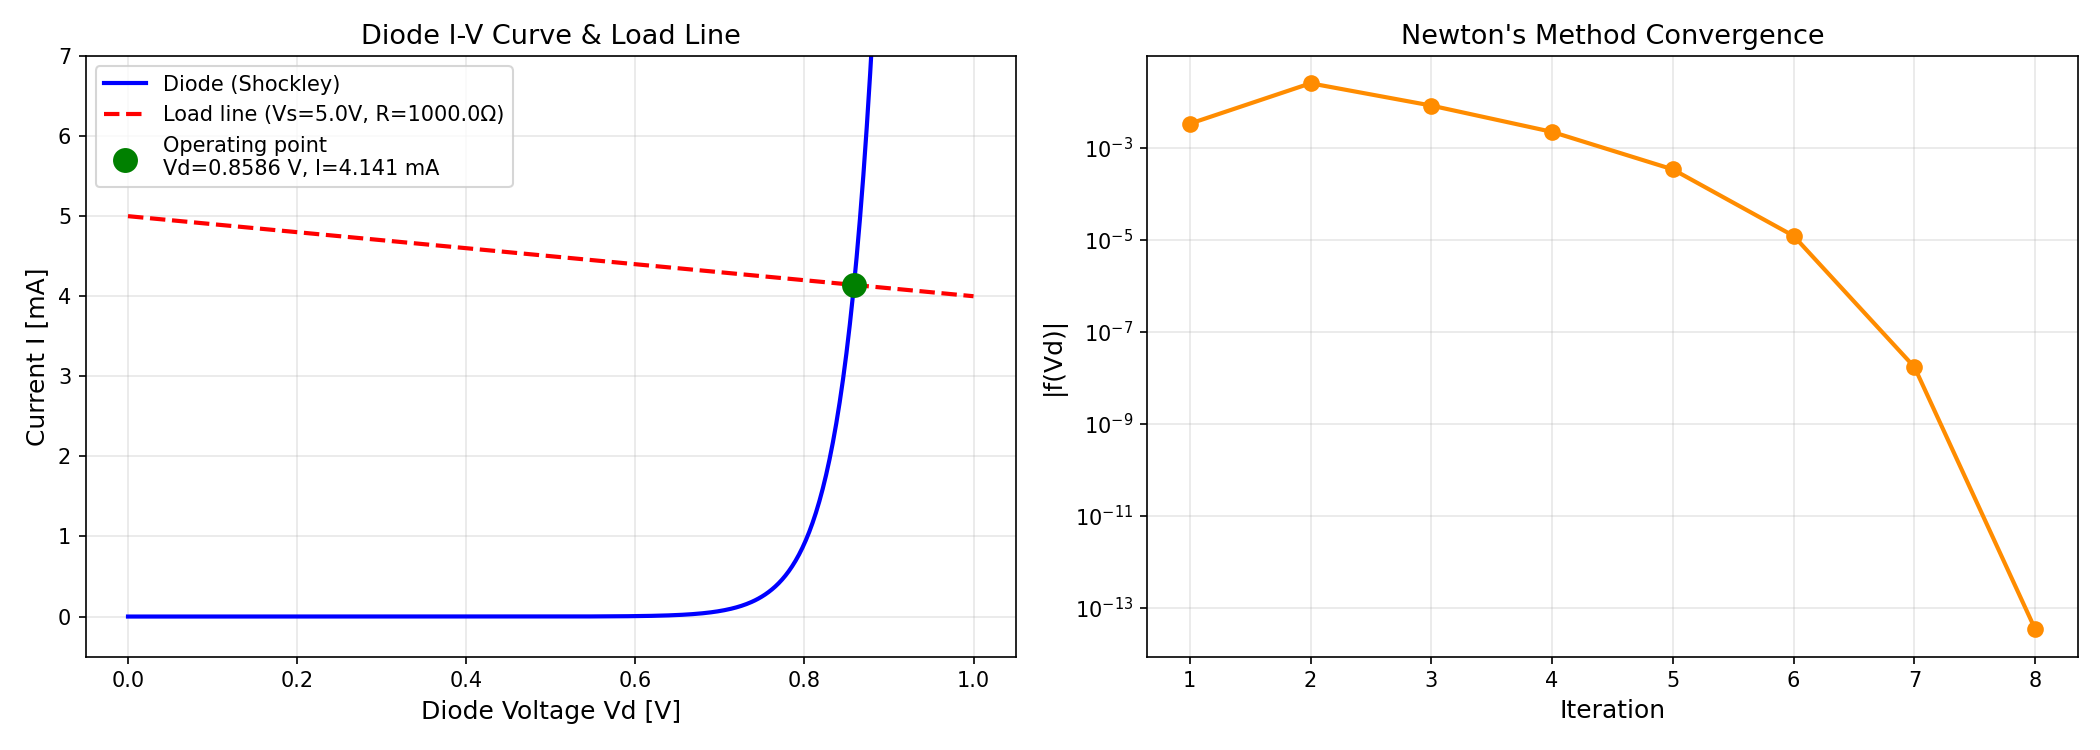
\includegraphics[width=\columnwidth]{newton_diode_results.png}
  \caption{Left: Diode I--V curve and load line with operating point.
           Right: Newton's method convergence ($|f(V_d)|$ vs.\ iteration).}
  \label{fig:iv}
\end{figure}

\subsection{Convergence Comparison}
Figure~\ref{fig:conv} compares the convergence of Newton's method and
bisection.  Newton's method (orange) reaches machine precision in roughly
8~iterations, exhibiting the characteristic steep drop of quadratic
convergence.  Bisection (blue) decreases linearly and requires approximately
50~iterations to reach the same tolerance.

\begin{figure}[H]
  \centering
  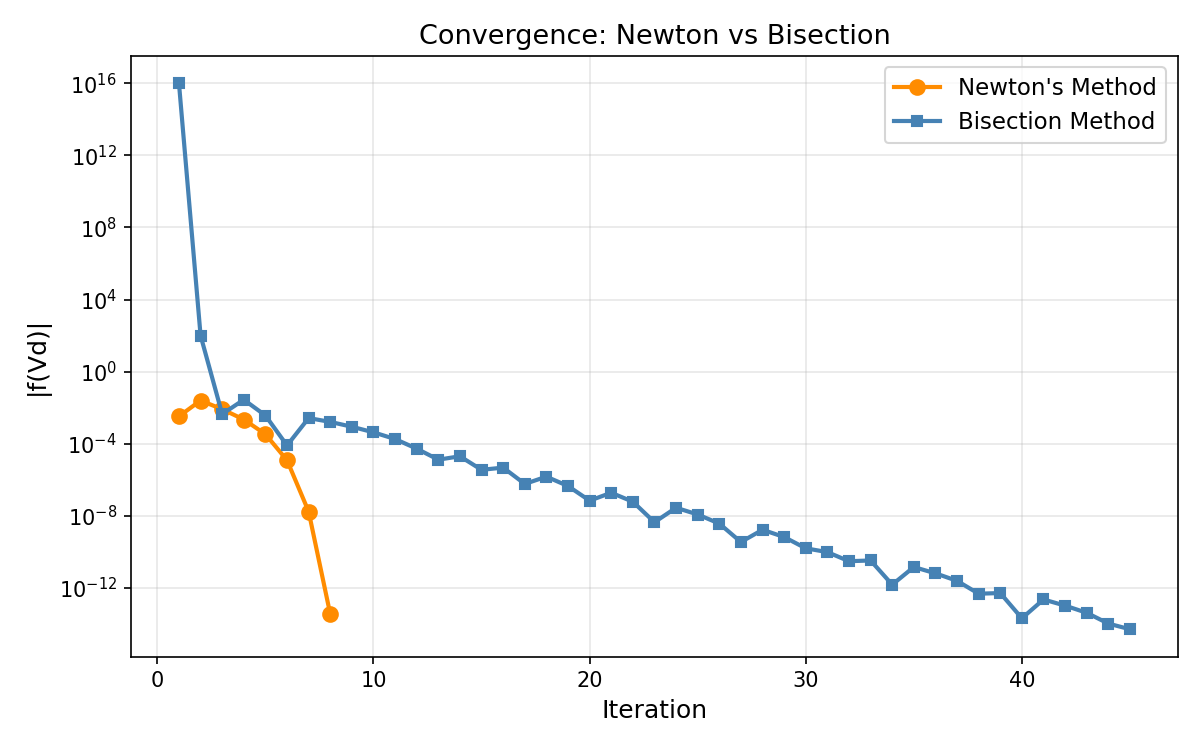
\includegraphics[width=\columnwidth]{newton_vs_bisection.png}
  \caption{Convergence comparison: Newton's method vs.\ bisection.}
  \label{fig:conv}
\end{figure}

% ════════════════════════════════════════════════════════════════════
\section{Discussion}

\subsection{Advantages of Newton's Method}
\begin{itemize}
  \item \textbf{Fast convergence:} Quadratic convergence means the number of
        correct digits roughly doubles each iteration.
  \item \textbf{Few iterations:} Only 8~iterations were needed to reach
        $|f| < 10^{-10}$.
  \item \textbf{No interval required:} Unlike bisection, Newton's method needs
        only a single starting point.
\end{itemize}

\subsection{Disadvantages of Newton's Method}
\begin{itemize}
  \item \textbf{Requires derivative:} The user must supply~$f'(x)$, which may
        be difficult or impossible to obtain analytically.
  \item \textbf{Sensitive to initial guess:} A poor starting point can cause
        divergence or oscillation, especially when $f'(x) \approx 0$.
  \item \textbf{No guaranteed convergence:} Unlike bisection, there is no
        guarantee that the method converges for arbitrary starting points.
\end{itemize}

\subsection{When to Use Each Method}
Use \textbf{bisection} when reliability is paramount, when derivatives are
unavailable, or when the initial guess is uncertain.  Use \textbf{Newton's
method} when the derivative is known, a reasonable initial guess is available,
and fast convergence is desired---as is typical in circuit simulation (e.g.,
SPICE uses Newton--Raphson iteratively to solve nonlinear device equations at
every time step).

% ════════════════════════════════════════════════════════════════════
\section{Conclusion}

We formulated the DC operating-point problem for a series diode circuit as a
single nonlinear equation and solved it using Newton's method.  The method
converged in 8~iterations to $V_d \approx 0.859\;\text{V}$,
$I \approx 4.14\;\text{mA}$, demonstrating the quadratic convergence that
makes it the preferred algorithm in circuit simulators worldwide.  A comparison
with bisection confirmed the dramatic difference in convergence speed.

\end{document}



\clearpage
%%%%%%%%%%%%%%%%%%%%%%%%%%%%%%%%%%%%
% Overall Document Guidelines: Head
%%%%%%%%%%%%%%%%%%%%%%%%%%%%%%%%%%%%
\section{Overall Document Guidelines: Head}
\label{sec:intro}

Clear document of any fonts other than Times, Arial, and Symbol. The
paper should be formatted using the tags provided in the template,
i.e., title, author, section, subsection, subsubsection, eq./fig.,
references, etc.  in a 2 column format on US letter size paper ($8.5
\times 11$ inches, or $21.6 \times 27.9$ cm).

The left and right margins are set automatically to .75 inch (1.90 cm),
and the top and bottom margins to 1.0 inch (2.54 cm). The document is in
a 2-column format with column widths set at 3.38 inch (8.57 cm) and the
gutter -the space between columns- at .25 inch (0.635 cm).

Papers should be a maximum of 4-6 pages; longer papers will be
returned for revision. Please do not place folios or page numbers in
your paper. That information is inserted when we assemble the book.


%%%%%%%%%%%%%%%%%%%%%%%%%%%%%%%%%%
% Graphics and Equations
%%%%%%%%%%%%%%%%%%%%%%%%%%%%%%%%%%
\section{Graphics and Equations}
Graphics and equations should fit within one column (3.38 inches
wide), but full width (7 inch) figures are also acceptable. Equations,
figures and figure captions each have their own style tags. Equations
are numbered using parentheses flushed right as shown below.

\begin{equation}
\label{eq:ist}
\textrm{IS\&T} + \textrm{members} \times \textrm{Confs.} = \textrm{Success}
\end{equation}


\subsection{Helpful Hints and Style Tags: Subhead}
For a complete listing of the style tags for use in this template
refer to Table \ref{tab:fonts}. These are the style tags for
conference proceedings; if you use the wrong template/style tags your
paper will be sent back to you to be reformatted.  All of these forms
and templates related to the publication of conference papers are
available at

www.imaging.org/conferences/guidelines.cfm. 

Select the specific conference and download the Authors Kit. The
template may vary from one conference to another.

The template is set up for MS Word and LaTeX. Please check the paper
carefully to confirm that the styles have been applied correctly, then
print it out and double check to ensure that the paper appears as
intended.

\begin{table}[!h]
\caption{Style Tag Table: Table head}
\label{tab:fonts}
\begin{center}       
\begin{tabular}{|p{0.45\columnwidth}|p{0.45\columnwidth}|} 
\hline
1. Title& title environment \\ \hline
2. Byline: & \\
Author/Affiliation & author environment \\ \hline
3. Head & section environment \\ \hline
4. Subhead & subsection environment \\ \hline
5. Tertiary head & subsubsection environment \\ \hline
6. Abstract & abstract environment \\ \hline 
& \\ \hline
7. Body & regular text\\ \hline
8. Equation & equation environment\\ \hline
9.1 Figure & align left \\ \hline
9.2 Figure caption & caption environment \\ \hline
10.1 Table head & caption environment \\ \hline
10.2 Table text & tabular environment \\ \hline
11. References & bibliography + 
command \emph{small} to have a 1pt smaller font\\ \hline
12. Author Bio text & biography environment\\ \hline
13.1 List, bullet & itemize environment\\ \hline
13.2 List, numbered & enumerate environment \\ \hline
\end{tabular}
\end{center}
\end{table} 

%%%%%%%%%%%%%%%%%%%%%%%%%%%%%%%%%%
% Submitting Your Paper
%%%%%%%%%%%%%%%%%%%%%%%%%%%%%%%%%%

\section{Submitting Your Paper}
The submission of your paper has to be performed through the IS\&T
submission website. Authors receive a login for this site by e-mail.
Papers can be submitted in Postscript, Word, or WordPerfect format,
and will be converted to PDF by the submission server. Please
carefully review the generated PDF and verify that all the text,
equations, figures and tables are displayed correctly before approving
its submission.

\subsection{Margins in LaTeX}
Because of the differences between dvips conversion utilities, the
margins of your generated PDF document might vary. Please print
your document, and verify its margins. If they are incorrect, please
adapt the sizes of the margins in the file \emph{ist.sty}. Typically the
top margin should be decreased.

\begin{table}[!h]
\caption{Document Specs: Table head}
\label{tab:specs}
\begin{center}       
\begin{tabular}{p{0.35\columnwidth}p{0.55\columnwidth}} 
Paper Size & US Letter \\
Left/right margin & .75 inch (1.90 cm) \\
Top/bottom margin & 1 inch (2.54 cm) \\
Columns & 2 at 3.38 inch (8.57 cm) wide. \\
 & Spacing between columns: 0.25 inch (0.635 cm)
\end{tabular}
\end{center}
\end{table} 

\begin{figure}[!hb]
  \includegraphics[width=0.3\columnwidth]{logo.png}
  \caption{IS\&T logo.}
  \label{Figure:logo}
\end{figure}

Please contact IS\&T with any questions or requests for assistance in
helping prepare the paper. We look forward to having your paper
presented at the conference and published in the conference
proceedings.

\begin{figure}[!hb]
  \includegraphics[width=0.3\columnwidth]{logo.png}
  \caption{IS\&T logo.}
  \label{Figure:logo}
\end{figure}

%%%%%%%%%%%%%%%%%%%%%%%%%%%%%%%%%%
% Reference Preparation
%%%%%%%%%%%%%%%%%%%%%%%%%%%%%%%%%%

\section{Reference Preparation}
Use the standard LaTeX \emph{cite} command for references in the
text. You can then use the standard bibliography command to generate
the list of references. Add the command \emph{small} before the
bibliography to give it the right font size.  Reference \cite{bib1}
style should be used for books, Reference \cite{bib2} style should be
used for Journals, and Reference \cite{bib3} style should be used for
Proceedings.

%\section{Acknowledgments} 
%add the acknowledgement section here

% To start a new column (but not a new page) and help balance the last-page
% column length use \vfill\pagebreak.

%%%%%%%%%%%%%%%%%%%%%%%%%%%%%%%%%%
% Bibliography
%%%%%%%%%%%%%%%%%%%%%%%%%%%%%%%%%%

\small
\begin{thebibliography}{9}
\bibitem{bib1}John Doe, Recent Progress in Digital Halftoning II,
  IS\&T, Springfield, VA, 1999, pg. 173.
\bibitem{bib2}John Doe, Digital Imaging, J. Imaging. Sci. and
  Technol., 42, 112 (1998).
\bibitem{bib3}John Doe, An Inexpensive Micro-Goniophotometry You Can
  Build, Proc. PICS, pg. 179. (1998).
\end{thebibliography}

%%%%%%%%%%%%%%%%%%%%%%%%%%%%%%%%%%
% Biography
%%%%%%%%%%%%%%%%%%%%%%%%%%%%%%%%%%

\begin{biography}
Please submit a brief biographical sketch of no more than 75 words. 
Include relevant professional and educational information as shown 
in the example below.

Jane Doe received her BS in physics from the University of Nevada (1977) 
and her PhD in applied physics from Columbia University (1983). Since 
then she has worked in the Research and Technology Division at Xerox 
in Webster, NY. Her work has focused on the development of toner adhesion 
and transport issues. She is on the Board of  IS\&T and a member of APS 
and SPIE.
\end{biography}

\end{document} 
